\chapter{Intro}\label{ch:intro}

In recent months and years, neural networks have produced many \textit{state-of-the-art} results in almost all possible disciplines of machine learning \cite{NTG2}. The roots of Neural Networks (NN) lie down almost 80 years ago in 1943, when \textbf{McCulloch-Pitts} \cite{NN} compared for the first time neuronal networks with the structure of the human brain. This first attempt to approach artificial neurons with neurons from the brain lead to the nowadays commonly used understanding of a simple neuron of a basic neural network (shown in figure \ref{neuron}). Those neurons connected together create an aritificial neuronal network, which can calculate any possible logical or arithmetic function. 

\begin{figure}
  \begin{center}
  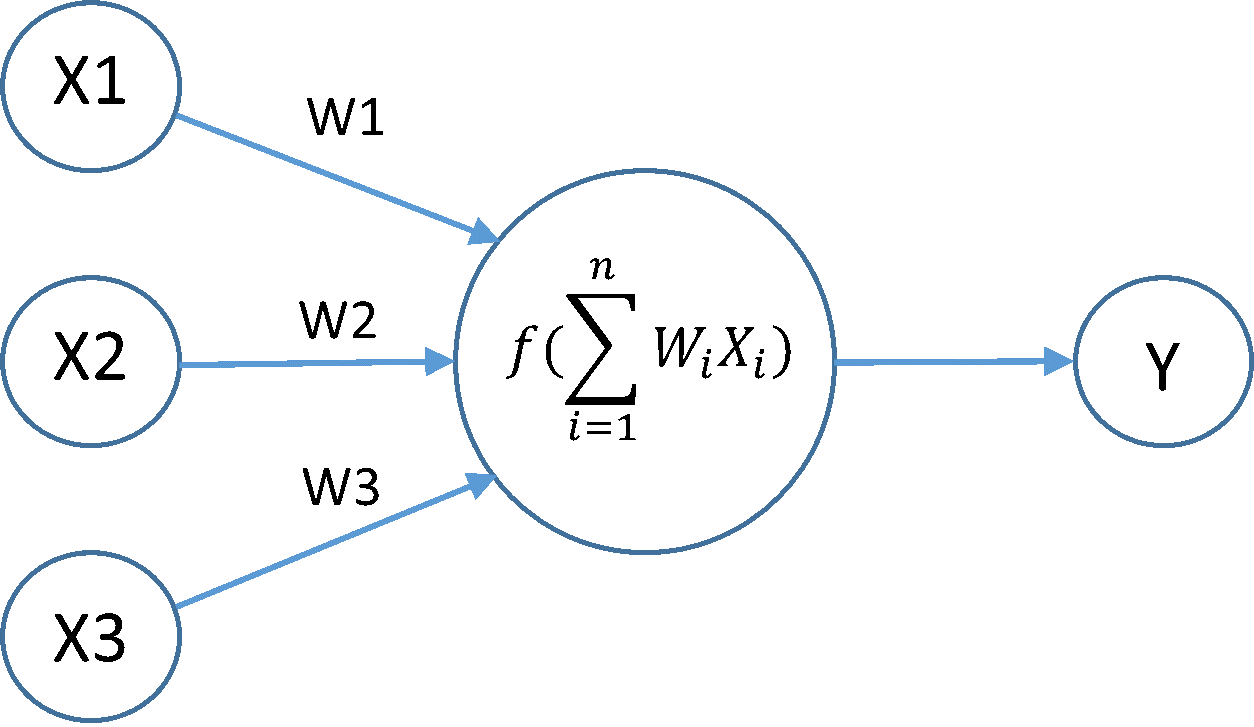
\includegraphics[width=3.5in]{photos/neuron}\\
  \caption{A simple Neuron with 3 inputs and 1 output \cite{neuron}}\label{neuron}
  \end{center}
\end{figure}

The range in which NN's (2020) can be applied nowadays is wide. Some disciplines have only been created due of the invention of neural networks, because they solve existing- and new problems very effective and efficiently. Many frequently held conferences around the globe contribute continuous evidence of the successes of neural networks. Among those various disciplines counts for example \textit{Pattern recognition} with Convolutional Neural Networks (CNN) \cite{cnn} or the famous \textit{CIFAR-10} dataset \cite{cifar}, where many amateurs \cite{tim} and experts attempt annually to further increase the accuracy of predicting the 10 different image classes. \\
The topic of this thesis \textit{textgeneration} is based from the Natural Language Processing discipline, \textit{NLP} for short. This field covers many other hot research topics, such as 

\begin{itemize}
\item Sentiment Analysis
\item Machine Translation
\item Voice Recognition
\item Text Generation (Neural Text Generation \textit{NTG})
\end{itemize}

Another term for textgeneration is denoted by \textit{Language Modelling}, because generators use the words and grammar as input for the model. In the past five years were mainly two approaches for modelling NLP, namely the \textbf{rule-based} system and the \textbf{template-based} system (Figure \ref{rules_based}) \cite{NTG2}. Today neural end-to-end systems are is \textit{State-of-the-Art} \cite{End_to_End}. These new systems offer more flexibility and scale with proportionately better results and less data is required, because the complexity and thus the neccessary computing power has increased. However, this fact leads to a complexity problem, because it becomes very difficult to understand the decisions of the neural network. The neural network is still to a large extent basically a \textit{black box}, although it gives surprisingly good results, especially in NLP. Nevertheless, neural network models for text processing are difficult to understand, so nowadays compromises between rule-based systems still have to be made and hybrid systems are most commonly used. 

\begin{figure}
  \begin{center}
  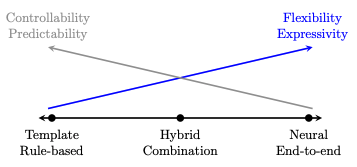
\includegraphics[width=3.5in]{photos/rule_based}\\
  \caption{Rule-Based vs. Neural-Text-Generations System \cite{NTG2}}\label{rules_based}
  \end{center}
\end{figure}

The neural text generation, also called \textit{NTG}, has many other interesting application fields, including
\begin{itemize}
\item Speech recording and conversion to text
\item Conversation systems e.g. chatbots
\item Text summary
\end{itemize} 

In order to train language models, they must be taught the probability of occurring words in relation to the preceding words. There are several approaches to achieve this goal. Language models can be trained on the level of words, whole sentences or even whole paragraphs. The granularity in which the training takes place is called \textit{n-grams}, where \textit{n} represents the number of preceding words.

\section{Case study of a current NLP system}



\subsection{Case study}

Image-to-Text | Captionbot Microsoft

\subsection{Useful application areas of NLP systems}

IoT, Grammerly, ok

\subsection{Useful application areas of NTG systems}

Grammerly